% supplemental.tex --- Supplemental Material (proofs), anonymized for
% double-anonymous review. S.1--S.6: proofs of Propositions 2--5, Lemma 1,
% and the full constructions for Proposition 1 (sketched in the main text).
% Compile: pdflatex supplemental (x2).
\documentclass[11pt,a4paper]{article}
\usepackage[margin=2.6cm]{geometry}
\usepackage{amsmath,amssymb,amsthm}
\usepackage[colorlinks=true,linkcolor=blue,citecolor=blue,urlcolor=blue]{hyperref}
\usepackage{booktabs}
\usepackage{graphicx}

\newtheorem*{proposition}{Proposition}
\newtheorem*{lemma}{Lemma}
\renewcommand{\thefigure}{S.\arabic{figure}}
\renewcommand{\thetable}{S.\arabic{table}}

\begin{document}

\title{Supplemental Material for\\ ``Structural rupture of rough dependency
graphs: relational anomaly detection in multivariate time series''}
\date{}
\maketitle

\noindent This document contains the proofs of Propositions 1--5 and
Lemma~1 of the main text (S.1--S.6), per-seed statistics with
uncertainty (S.7), calibration and implementation details including the
provenance of every hyperparameter (S.8), threats to validity and the
guarantee boundary (S.9), the full trace of the gas-pipeline case study
(S.10), a plain-language notation glossary (S.11), per-type results
aggregated from the frozen per-seed files (S.12), the robustness
audit of the copula-standardisation constants on synthetic and real
networks (S.13), a longer-training audit of the deep arms (S.14),
scaling measurements of construction versus online cost (S.15), a
practitioner's selection guide (S.16), a window-level view of the
case attacks in the plane of the dependency degree and direction
(S.17), data and configuration provenance (S.18), a random-host
injection audit beyond the candidate graph (S.19), and a scope probe
on value-dominant public benchmarks (S.20). Main-text proof
sketches point here; the proof correspondence is:

\medskip
\noindent\begin{tabular}{@{}ll@{}}
\toprule
Item & Main-text statement \\
\midrule
S.1 & Proposition 2 (bounds and extrema of $\gamma$) \\
S.2 & Proposition 3 (crisp-table correspondence with the Pawlak degree) \\
S.3 & Proposition 4 (inversion invariance of $\gamma$) \\
S.4 & Proposition 5 (monotonicity under decision-granule coarsening) \\
S.5 & Lemma 1 (margin-preserving injections) \\
S.6 & Proposition 1 (complementary blind spots; full constructions) \\
\bottomrule
\end{tabular}
\medskip

\noindent Notation follows the main text: $\pi$ is a copula-standardised
granular decision table over $K$ decision granules, $\pi_g$ the occupancy
of condition granule $g$, $\pi_{v\mid g}$ its conditional decision
distribution, $c_g=\max_v \pi_{v\mid g}$ the row confidence, and
$\gamma(\pi)=\sum_g \pi_g c_g$ the occupancy-weighted modal rule
confidence.

\section*{Notation and proof conventions}

Three conventions are used throughout the proofs. First, \emph{raw versus
smoothed tables}: $\pi_{\mathrm{raw}}(T)$ denotes the unsmoothed empirical
granular table, and $\pi_{\mathrm{sm}}$ the operational table after one
additive-smoothing pass ($\alpha$ counts) and iterative proportional
fitting to uniform margins; exact correspondences with the Pawlak degree
are stated for $\pi_{\mathrm{raw}}$, and the main text (C1) quantifies how
$\gamma(\pi_{\mathrm{sm}})$ approaches them. Second, \emph{perturbation
size}: $\epsilon$ always denotes the total-variation size of a local
conditional-law perturbation, and divergence responses are stated in
these units (with second-order Jensen--Shannon response on tables with
positive cells). Third, \emph{recoding maps}: inversions are modelled as
the order-reversing permutation $r(v)=K-1-v$ of the decision granules,
under symmetric quantiles; arbitrary bijections are not claimed. The
margin-preservation lemma covers per-channel scores and threshold
exceedance counts inside the injection window; gap-merged run counts and
false-alarms-per-day functionals lie outside its scope and are always
reported as measured.

\section*{S.1 Proof of Proposition 2 (bounds and extrema)}

\begin{proposition}[Bounds and extrema]
Let $\pi$ be a copula-standardised granular table over $K$ decision granules.
Then $1/K \le \gamma(\pi) \le 1$. Also $\gamma(\pi)=1$ iff every occupied
row is deterministic (all mass concentrated in one decision granule), and
$\gamma(\pi)=1/K$ iff every occupied row is uniform over the $K$ decision
granules.
\end{proposition}

\begin{proof}
Write $c_g=\max_v \pi_{v\mid g}$ for the conditional confidence of row $g$.
Since $\pi$ has uniform margins, $\sum_g \pi_g = 1$, and
$\gamma = \sum_g \pi_g c_g$ is a convex combination of the $c_g$. For each
occupied row, $1/K \le c_g \le 1$ (the conditional distribution is a
probability vector on $K$ classes), hence $1/K \le \gamma \le 1$. Equality on
the right requires $c_g=1$ for every row with $\pi_g>0$, i.e.\ each occupied
row is concentrated in a single decision granule; equality on the left
requires $c_g = 1/K$, i.e.\ every occupied row is uniform.
\end{proof}

\section*{S.2 Proof of Proposition 3 (crisp-table correspondence)}

\begin{proposition}[Crisp-table correspondence with the Pawlak degree]
Let $T$ be a decision table in which every granule $g$ induces a constant
decision (a crisp decision subtable after granulation), and let
$\pi_{\mathrm{raw}}(T)$ be its unsmoothed empirical granular table. Then the
Pawlak positive region is $POS(T)=\{t:\ \text{the granule of } t \text{ is
deterministic}\}$, the classical degree is
$\gamma_P(T)=|POS(T)|/|U|$, and $\gamma(\pi_{\mathrm{raw}}(T))=\gamma_P(T)$.
In general, for $\beta\in(0,1]$ and any granular table $\pi$, the
variable-precision degree
$\gamma_\beta=\sum_{g:\,c_g\ge\beta}\pi_g$ counts rows whose confidence
reaches $\beta$, and
$\gamma(\pi)=\sum_g \pi_g c_g \ge \beta\,\gamma_\beta$, with equality iff
every occupied row has confidence exactly $\beta$.
\end{proposition}

\begin{proof}
In a crisp subtable, every occupied row has $c_g=1$, so
$\gamma=\sum_{g}\pi_g c_g=\sum_g \pi_g$ over the deterministic rows. Since
$POS(T)$ is precisely the union of deterministic granules and
$\pi_g=|g|/|U|$, $\gamma=\sum_{g \text{ det.}} |g|/|U| = |POS(T)|/|U| =
\gamma_P(T)$. For the inequality, write
$\gamma-\beta\gamma_\beta
=\sum_{c_g\ge\beta}\pi_g(c_g-\beta)
+\sum_{c_g<\beta}\pi_g c_g$;
both sums are non-negative, the first vanishes iff every counted row has
$c_g=\beta$ exactly, and the second vanishes only if no occupied row has
$c_g<\beta$ (occupied rows have $c_g\ge 1/K>0$). Equality therefore
requires every occupied row to be counted with $c_g=\beta$ exactly.
\end{proof}

\section*{S.3 Proof of Proposition 4 (inversion invariance)}

\begin{proposition}[Inversion invariance of $\gamma$]
Let the pair $(x_i, x_d)$ satisfy a deterministic relation with granule map
$\varphi$ (i.e.\ $x_d$'s granule is a function $\varphi$ of $x_i$'s
granule), and let the output channel be re-encoded by an order-reversing
permutation of its granules, $r(v)=K-1-v$ (with symmetric quantiles,
granulation commutes with this recoding). Then $\gamma$ is unchanged,
$\rho$ drops by the mass of the rows whose modal rule changed (to its
floor when every occupied row changes), $|\delta|$ is unchanged, and the
sign of $\delta$ flips.
\end{proposition}

\begin{proof}
The recoding permutes the decision columns of the granular table by the
order-reversing map $r$. A column permutation moves each row's mass to the
recoded column: each occupied row still concentrates all mass in a single
column, so $c_g=1$ and the occupancy $\pi_g$ is unchanged; hence
$\gamma=\sum_g\pi_g c_g$ is unchanged. The modal map becomes
$r\circ\varphi$; the agreement indicator in $\rho$ vanishes on rows where
$r\circ\varphi\neq\varphi^{\mathrm{ref}}$, so $\rho$ falls by the mass of
exactly those rows. The centre-centred correlation
$\delta$ is an odd functional of the column map: composing with the
order-reversing map $r(v)=K-1-v$ flips its sign while preserving
magnitude.
\end{proof}

\section*{S.4 Proof of Proposition 5 (coarsening monotonicity)}

\begin{proposition}[Monotonicity of $\gamma$ under decision-granule coarsening]
Let $\pi$ be a granular decision table over $K$ decision granules, with row
occupancies $\pi_g$ ($\sum_g \pi_g = 1$) and conditional rows
$\pi_{\cdot\mid g}$. Let $T'$ be the coarsened table obtained by replacing
the decision granules by a partition of them into $K' < K$ groups, leaving
the condition granules untouched, so that
$\pi'_{v'\mid g} = \sum_{v \in C_{v'}} \pi_{v\mid g}$ and $\pi'_g = \pi_g$.
Then $\gamma(\pi') \geq \gamma(\pi)$, with equality if and only if in every
occupied row no coarsened group carries more mass than the row's modal
column, that is
$\max_{v'} \sum_{v \in C_{v'}} \pi_{v\mid g} = \max_v \pi_{v\mid g}$.
\end{proposition}

\begin{proof}
For each occupied row $g$ the coarsened confidence is
$\max_{v'} \pi'_{v'\mid g} = \max_{v'} \sum_{v \in C_{v'}} \pi_{v\mid g}$.
The group $C^\ast$ containing the row's modal column $v^\ast$ satisfies
$\sum_{v \in C^\ast} \pi_{v\mid g} \geq \pi_{v^\ast\mid g} = \max_v \pi_{v\mid g}$,
so no row confidence decreases; the occupancies $\pi_g$ are unchanged, and
$\gamma = \sum_g \pi_g c_g$ is a non-negative combination of row
confidences. Row-level equality, $c'_g = c_g$, holds exactly when no group
sum exceeds the modal column mass. Two conditions are jointly required.
The modal group must not pool mass from outside the modal column: if it
did, its sum would be strictly larger than $\pi_{v^\ast\mid g}$ (a row of
$.6/.4/0$ with groups $\{v_1,v_2\},\{v_3\}$ coarsens confidence $.6$ to
$1.0$). And no other group may exceed the modal column's mass: a row of
$.4/.35/.25$ with groups $\{v_1\},\{v_2,v_3\}$ keeps the modal group clean
yet coarsens confidence $.4$ to $.6$. Since $\pi_g>0$ on occupied rows,
$\gamma$ is a convex combination of the row confidences with strictly
positive weights, so the global equality holds if and only if the row-level
equality holds in every occupied row.
\end{proof}

\section*{S.5 Proof of Lemma 1 (margin-preserving injections)}

\begin{lemma}[Margin-preserving injections]
Fix a window $W$ and a target channel $j$. Any injection that outputs a
permutation of the observed values $\{x_j(t)\}_{t\in W}$ leaves the empirical
marginal distribution of $j$ (and of every other channel) unchanged
point-wise. Consequently, for any detector whose per-time score is a fixed function of the
single-channel value (any model or normalisation being fitted strictly
outside the window; scores that pair the target with another channel, such
as prediction residuals, are not covered), the multiset of scores over $W$ is unchanged by
the injection, hence so is the number of threshold exceedances inside $W$
and the indicator that at least one exceedance occurs in $W$. Detection rates that depend only on these window-level exceedance
counts (for example detecting a window event by requiring
at least one exceedance inside it) are therefore unchanged. Gap-merged event-level
metrics are not claimed invariant (merging can regroup exceedances across
window boundaries); the experimental event recalls are reported as measured.
\end{lemma}

\begin{proof}
A permutation of a multiset leaves its order statistics, and therefore the
empirical distribution function, identical at every point. A per-channel
score function $s_j(x_j(t))$ thus produces an identical multiset of scores
$\{s_j(x_j(t)): t\in W\}$ before and after the injection. For any threshold,
the number of exceedances inside $W$ is a function of that multiset alone,
and the permutation maps alarm times inside $W$ to times that remain inside
$W$; so the number of exceedances in $W$, and whether at least one occurs
there, are both unchanged. Per-window exceedance counts and indicators are unchanged; all
event-level metrics under any matching convention, and any aggregation
across channels, are outside the lemma.
Two quantities are \emph{not} claimed invariant: the time stamps of the
crossings may move within $W$, and the number of distinct gap-merged events
can change (a permutation may split or merge alarm runs), so event-count
functionals such as false events per day are not exactly
permutation-invariant; the empirical floor results of the main text's
capability-gate and injection-suite experiments are therefore reported as
measured rather than deduced. Isolation Forest and LOF scores are functions of the
single-channel value at each time (model fitted outside the window);
window-based divergence monitors (correlation, partial correlation, MI) are
\emph{not} so restricted and are likewise evaluated empirically rather than
covered by the lemma.
\end{proof}

\section*{S.6 Proof of Proposition 1 (complementary blind spots)}

\begin{proof}
(i) Inversion $Y=X \mapsto Y=-X$. Take symmetric reference quantiles so that
granulation commutes with negation ($g(-x)=K-1-g(x)$). The injected table is
the reference table with columns reversed; margins are unchanged, so
$\pi$ is unchanged up to the column permutation, the row confidences
$c_g$ are unchanged, and $\gamma$ is unchanged. The modal map becomes
$v\mapsto K-1-v$; where the reference map was the identity, $\rho$ drops by
the mass of the moved rows, and $\delta$ flips sign (order-reversing
bijection). So $\gamma$ alone cannot distinguish this inversion from no
change, whereas $(\rho,\delta)$ do.

(ii) Conditional reshaping. Let $\epsilon$ denote the total-variation size
of the perturbation of the conditional law of a single granule $g^\ast$
(occupied mass $\pi_{g^\ast}>0$), with every row's modal decision and
occupancy kept fixed. $\gamma$ changes by at most $\pi_{g^\ast}\cdot
O(\epsilon)$ (the modal confidence is pinned), while the conditional
distribution of $g^\ast$ moves by $\Theta(\epsilon)$ in total variation.
Because the $\alpha$-smoothed cells of the standardised table are strictly
positive, the Jensen--Shannon divergence of that row is second order in
the perturbation: $D_{JS}$ moves by $\Theta(\pi_{g^\ast}\epsilon^2)$.

(iii) Subset-joint emergence. Let $x_d=f(x_{i_1},x_{i_2})$ with $f$ the
parity (exclusive-or) of the two parents' binary granules, the parents
independent and uniform on their two granule values. Every pair table has
independent margins and $\Pr(g_d\,|\,g_{i_1})$ uniform over the two values of $g_d$,
so no pair-edge statistic moves off its null value ($\rho$ compares
the reference and current noise modal maps, which coincide in the
population construction). The subset edge
$((i_1,i_2),d)$ has rows that are deterministic, so $\gamma=1$.

Constructions (i)-(iii) give: $\gamma$ blind to inversion (i) and
bounded at order $\pi_g\epsilon$ under reshaping (ii), with neither $\rho$ nor $\delta$ constrained by (ii); and every pair-level
statistic blind to the subset-joint construction (iii), which the subset
edge recovers. No single pair-level component therefore covers the three
canonical changes.
\end{proof}

\section*{S.7 Per-seed results and uncertainty}

Table~\ref{tab:suppseed} lists the per-seed event recall and realised
false-alarm rate of the full detection family and its $\gamma$-only
ablation on the three real networks, with the matched-pairs rank-biserial
effect size for the paired comparison.
Table~\ref{tab:suppci} reports bootstrap recall confidence intervals
(per-seed resampling) and mean realised false-alarm rates for the main
methods. These summaries are derived from the frozen per-seed result
files by a single script; no new experiments are involved.

\medskip
\noindent\textbf{Selection-adjusted significance.} The per-network
``strongest external baseline'' is selected post hoc among the eleven
external baselines, so the headline comparisons carry a multiplicity
burden beyond the Holm correction across networks reported in the main
text. We therefore re-tested them with the Westfall--Young single-step
min-P procedure over the eleven per-network paired comparisons, using
exact sign-flip enumeration of the per-seed recall differences
($2^{10}=1024$ flips). The advantage over the strongest external
baseline remains significant on METR-LA (adjusted $p=0.001$) and
PEMS-BAY (adjusted $p=0.002$); on Beijing-Air the comparison family
contains decisively significant members (family min-P adjusted
$p=0.003$) but the strongest external baseline is not among them,
consistent with the main text's reporting (frozen script
\texttt{gen\_select\_adjusted.py}, frozen JSON
\texttt{e2\_select\_adjusted.json}).

\begin{table}[h]\centering\small
\caption{Per-seed event recall and realised false alarms per day
(full family vs.\ $\gamma$-only ablation), ten seeds per network.}
\label{tab:suppseed}
\begin{tabular}{lccccc}
\hline
Network & Seed & RDSG & FA/d & $\gamma$-only & FA/d \\
\hline
METR-LA & 1 & 0.46 & 0.21 & 0.33 & 0.22 \\
 & 2 & 0.52 & 0.11 & 0.37 & 0.19 \\
 & 3 & 0.50 & 0.14 & 0.21 & 0.27 \\
 & 4 & 0.46 & 0.21 & 0.29 & 0.27 \\
 & 5 & 0.48 & 0.13 & 0.44 & 0.18 \\
 & 6 & 0.36 & 0.19 & 0.40 & 0.19 \\
 & 7 & 0.48 & 0.14 & 0.24 & 0.24 \\
 & 8 & 0.38 & 0.19 & 0.38 & 0.22 \\
 & 9 & 0.48 & 0.13 & 0.40 & 0.16 \\
 & 10 & 0.44 & 0.16 & 0.41 & 0.22 \\
 & mean & 0.46 & 0.16 & 0.35 & 0.22 \\
 & \multicolumn{5}{l}{rank-biserial $r$ (RDSG vs $\gamma$-only): 0.87} \\
\hline
Beijing-Air & 1 & 0.22 & 0.02 & 0.39 & 0.02 \\
 & 2 & 0.26 & 0.01 & 0.21 & 0.02 \\
 & 3 & 0.21 & 0.01 & 0.29 & 0.01 \\
 & 4 & 0.23 & 0.01 & 0.27 & 0.02 \\
 & 5 & 0.14 & 0.01 & 0.19 & 0.02 \\
 & 6 & 0.16 & 0.01 & 0.24 & 0.01 \\
 & 7 & 0.30 & 0.01 & 0.40 & 0.01 \\
 & 8 & 0.33 & 0.01 & 0.33 & 0.01 \\
 & 9 & 0.25 & 0.01 & 0.35 & 0.02 \\
 & 10 & 0.17 & 0.02 & 0.22 & 0.01 \\
 & mean & 0.23 & 0.01 & 0.29 & 0.01 \\
 & \multicolumn{5}{l}{rank-biserial $r$ (RDSG vs $\gamma$-only): -0.87} \\
\hline
PEMS-BAY & 1 & 0.48 & 0.19 & 0.44 & 0.13 \\
 & 2 & 0.59 & 0.10 & 0.52 & 0.06 \\
 & 3 & 0.60 & 0.13 & 0.44 & 0.14 \\
 & 4 & 0.54 & 0.18 & 0.42 & 0.16 \\
 & 5 & 0.57 & 0.13 & 0.46 & 0.11 \\
 & 6 & 0.56 & 0.16 & 0.56 & 0.10 \\
 & 7 & 0.58 & 0.16 & 0.54 & 0.11 \\
 & 8 & 0.67 & 0.16 & 0.54 & 0.11 \\
 & 9 & 0.52 & 0.14 & 0.52 & 0.10 \\
 & 10 & 0.64 & 0.13 & 0.48 & 0.11 \\
 & mean & 0.57 & 0.15 & 0.49 & 0.11 \\
 & \multicolumn{5}{l}{rank-biserial $r$ (RDSG vs $\gamma$-only): 1.00} \\
\hline
\end{tabular}
\end{table}

\begin{table}[h]\centering\small
\caption{Bootstrap recall confidence intervals and mean realised
false-alarm rate by method and network.}
\label{tab:suppci}
\begin{tabular}{llccc}
\hline
Network & Method & Recall & 95\% CI & FA/d \\
\hline
METR-LA & RDSG & 0.46 & [0.42, 0.48] & 0.16 \\
 & IF-agg & 0.07 & [0.03, 0.12] & 0.13 \\
 & LOF-agg & 0.04 & [0.02, 0.06] & 0.13 \\
 & partial corr & 0.11 & [0.09, 0.14] & 0.10 \\
 & corr-matrix & 0.07 & [0.05, 0.09] & 0.06 \\
\hline
Beijing-Air & RDSG & 0.23 & [0.19, 0.26] & 0.01 \\
 & IF-agg & 0.00 & [0.00, 0.00] & 0.01 \\
 & LOF-agg & 0.00 & [0.00, 0.00] & 0.00 \\
 & partial corr & 0.24 & [0.23, 0.26] & 0.01 \\
 & corr-matrix & 0.18 & [0.16, 0.20] & 0.00 \\
\hline
PEMS-BAY & RDSG & 0.57 & [0.54, 0.61] & 0.15 \\
 & IF-agg & 0.00 & [0.00, 0.01] & 0.01 \\
 & LOF-agg & 0.49 & [0.46, 0.52] & 0.42 \\
 & partial corr & 0.03 & [0.01, 0.04] & 0.08 \\
 & corr-matrix & 0.00 & [0.00, 0.01] & 0.04 \\
\hline
\hline
\end{tabular}
\end{table}

Table~\ref{tab:supppaired} reports the paired per-seed recall difference
against the strongest external baseline on each network, with bootstrap
confidence intervals for the mean difference. The intervals quantify the main-text finding: RDSG is significantly
stronger than the strongest external baseline on METR-LA ($+0.268$ over
the compact Anomaly-Transformer arm) and on PEMS-BAY ($+0.086$ over the
LOF aggregation); on Beijing-Air the paired difference is $-0.013$ and
the interval crosses zero, matching the non-significant Wilcoxon p-value
in the main text (the partial-correlation divergence is nominally ahead
there). We note that the network
comparisons are made at the common \emph{requested} false-alarm budget
(realised rates differ, Table~\ref{tab:suppci}). Per-seed operating-curve
sweeps for every method ship with the reproduction package
(\texttt{results/paper/e2\_oc.json}); under event-counted matching at
$0.25$/day the windowed scorers gain most, consistently with boundary-window blobbing
(Section~5.3 of the main text), with GDN reaching $0.597$ on PEMS-BAY
against $0.579$ for RDSG, the metric arbitrage discussed there.

\begin{table}[h]\centering\small
\caption{Paired per-seed recall difference (RDSG $-$ strongest external
baseline) with bootstrap 95\% CI for the mean difference (10,000
resamples).}
\label{tab:supppaired}
\begin{tabular}{llcc}
\hline
Network & Baseline & Mean diff. & 95\% CI \\
\hline
METR-LA & Anomaly Trans. & +0.268 & [+0.191, +0.334] \\
Beijing-Air & partial corr & -0.013 & [-0.053, +0.030] (CI crosses zero) \\
PEMS-BAY & LOF-agg & +0.086 & [+0.036, +0.131] \\
\hline
\end{tabular}
\end{table}

\clearpage
\section*{S.8 Calibration and implementation details}

Values below are the frozen defaults of the main text (Table 3 there).
\emph{Standardisation:} one additive-smoothing pass with $\alpha=8$
counts, then two iterations of iterative proportional fitting towards
uniform margins; sparse rows therefore shrink towards uniform rather than
amplifying sampling noise. The independence floor of the exactly
standardised table is $1/K$; with two IPF iterations an independent table
still deviates slightly (up to $\gamma\approx0.28$ on sparse independent
tables at $K{=}4$, measured across 20 random constructions), which we
treat as the null floor in calibration. The deviation is a property of the
smoothing pass, not of the iteration count: running the same transform to
convergence (10{,}000 iterations) leaves the floor shift unchanged to the
seventh decimal (verified on skewed independent tables), so additional IPF
iterations cannot remove it and the calibration absorbs it by construction.
The family's boundary grid is the union of its $(K,w)$
configuration grids (16-point cadence on the 5-minute networks); the
rolling-update path of Table 3 uses $b=32$, and the rolling-mean
aggregator is a library option not exercised by the evaluated family scan.
The two channel monitors (R and E) are each calibrated at the full
requested budget; the union monitor's realised FA/day is the reported
operational quantity (Table 5).
\emph{Granularity:} $K=4$ equal-frequency granules per channel; detection
window $w=128$ points; stride and block length $b=32$. \emph{Candidate
graph:} the rupture channel keeps the top-16 reference-significant pairs,
the emergence pool the bottom-24 weak pairs plus, for each weak target,
subset edges over its $m{=}6$ closest weak partners; default
edge count $E=116$. \emph{Calibration:} every method's alarm thresholds are the \emph{smallest}
values whose reference self-scan alarm-sample rate meets the requested
false-alarm budget (samples counted at the method's native scoring
resolution; the merged-event FA/day reported in the tables is an
operational diagnostic, not the budgeted quantity), with block permutation
($b=32$, $B=499$) providing the nulls; attribution after an alarm uses Benjamini--Hochberg
control over the family. \emph{Event formation:} the RDSG family merges
alarms with a gap tolerance of 512 points (four windows) on the 5-minute
networks and 256 points on the hourly network; the window-divergence, VAR,
Granger and MI baselines merge at 256 points, the point aggregations and GDN
at 128. Overall recall uses pooled one-to-one matching over full event sets;
per-type recalls condition the true set on the event type and match against
all predicted events. \emph{Rolling update:} the
detector maintains a rolling buffer of $w/b$ granulated blocks per edge
and rebuilds each contingency table from the buffer at every boundary.

\medskip
\noindent\textbf{Provenance of the defaults.} No default in Table~3 of
the main text was chosen with knowledge of any real test segment. The
structural values were fixed once on the synthetic gate: $K{=}4$ and
$w{=}128$ sit inside the sensitivity grid of the main text's \S5.6
(default within $0.06$ of the best cell), and the edge budgets
$m_s{=}16$, $m_w{=}24$ follow the gate system's true structure (seven
genuinely strong unordered pairs and a twelve-pair weak group). The
block length $b{=}32$ is window geometry ($w/4$). The standardisation
constants are untuned design defaults: the smoothing strength
$\alpha{=}8$ and the two IPF iterations were chosen so that sparse rows
shrink towards uniform rather than amplifying sampling noise, and no
real-dataset feedback entered their choice; their robustness is audited
in S.13. The remaining constants are conventions: $B{=}499$ block
permutations (an odd count near 500 for stable null quantiles), the
BH level $q{=}0.05$, the maxT alarm level $\alpha_{\max}{=}0.01$, the
self-scan pruning cap $z_{\mathrm{prune}}{=}5.5$ retained from the gate's
unit-validity rule, and the (unexercised) rolling-mean length
$k_{\mathrm{roll}}{=}4$.

\section*{S.9 Threats to validity}

The ten seeds per network are injection repetitions on a single network
segment, not ten independent networks: the Wilcoxon and bootstrap analyses
quantify seed-to-seed stability under the injection protocol, not
cross-network evidence. A budget defined on a common time grid or on
alarm-duration fraction is a natural robustness variant; the shipped
sweeps support the common-grid reading directly.

The main text addresses each threat inline; we collect the mapping here.
\emph{Construct validity:} the injection suite is margin-preserving by
construction (Lemma~1), so it tests the relational blind spot only and
does not certify performance on anomalies that also move marginals; the
gas-pipeline section therefore treats the labelled attacks (50 of 53 with
a point footprint) as evidence of complementarity, not substitution.
\emph{External validity:} RDSG's advantage over the strongest external baselines is significant on
METR-LA and PEMS-BAY and not on Beijing-Air
(Table~\ref{tab:supppaired}); the significant advantage concentrates on
strong-association, lower-association hosts and short references.
\emph{Calibration validity:} thresholds are calibrated on a reference
segment whose length and stationarity bound the achievable false-alarm
control; attack-dense logs without quiet stretches defeat rolling
recalibration, as the gas analysis shows. \emph{Statistical validity:}
all headline numbers on the three injection networks are pooled over ten seeds (the WADI evaluation is a single labelled split without injection seeds) with Wilcoxon tests,
rank-biserial effect sizes, and bootstrap intervals
(Table~\ref{tab:suppseed}, Table~\ref{tab:supppaired}); all learned baselines (GDN and the compact AT/TranAD arms) train under
resource-constrained budgets (six and five epochs) that may under-train
them and could advantage RDSG, which is why
its comparison is reported per-method rather than pooled. S.14 closes
the question empirically: longer-training, larger-capacity versions of
both arms leave the ordering unchanged.

\medskip
\noindent\textbf{What is guaranteed and what is not.} For a reader
weighing the theoretical claims, the boundary is: Proposition~2's exact
independence floor $1/K$ holds on the \emph{exactly} standardised table;
the two-iteration IPF implementation approximates it (measured deviation
in S.8). The self-scan calibration delivers an empirical false-alarm
budget \emph{on the reference segment}; it is not a distribution-free
test-time guarantee, and thresholds migrate when the test segment
departs from the reference (the operating-curve analysis). The block
permutation nulls assume block exchangeability under stationarity of the
reference. Lemma~1 covers fixed single-channel value scores and
within-window threshold-exceedance counts; it does not cover pairing
residuals, learned monitors, or gap-merged event counts (FA/day). The
event type label remains an auxiliary summary (\S5.3 of the main text),
not a validated diagnostic.

\section*{S.10 Gas-pipeline case study: full trace}

Figure~\ref{fig:s10} plots the rolling three-statistic trace of the
case-study edge (setpoint$\to$gain, lag $-1$) over the full gas-pipeline
test segment, with all 53 labelled attacks shaded and the case attack
(the attack labelled $1{+}2{+}4{+}5{+}7$, yellow band) highlighted.
Windows of $w{=}128$ points slide in steps of 64; each window's table is
standardised exactly as in the pipeline ($\alpha{=}8$ smoothing, two IPF
iterations, blocks of 32), and $\gamma$ and $\delta$ are read
per-window while $D_{JS}$ is taken against the reference table. The
dotted lines mark the reference values ($\gamma=0.48$, $\delta=+0.28$);
the bold annotations at the case window are the values quoted in the
main text ($\gamma$ holds at $0.50$, $\delta$ reverses to $-0.34$,
$D_{JS}$ peaks at $0.23$). The figure script asserts, before plotting,
that the case window's unrounded statistics reproduce the frozen
case-study values to $10^{-9}$. Reproduction: MSU Gas Pipeline
\texttt{MainDataset.csv}, LOCF on process channels, reference segment
$[238860, 240480)$, events from 60-sample windows at attack density
$\ge 0.3$ merged at gap $\le 2$ windows;
\texttt{experiments/fig\_s10\_gas\_case.py} in the repository.

\begin{figure}[h]\centering
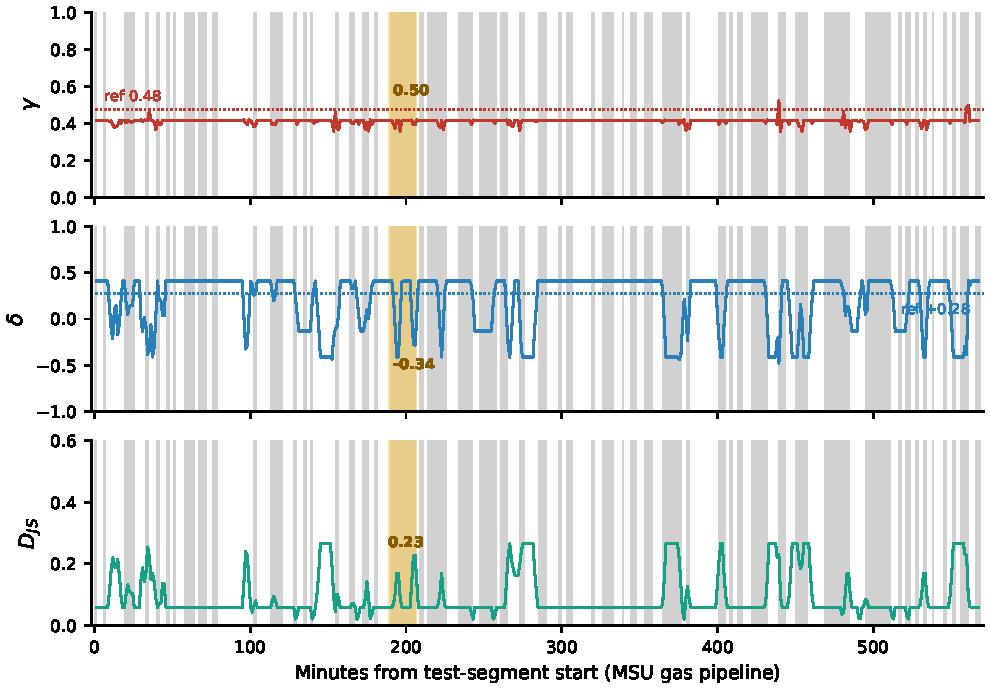
\includegraphics[width=\linewidth]{figs/s10_gas_case.pdf}
\caption{Case-study edge (setpoint$\to$gain): rolling $\gamma$, $\delta$
and $D_{JS}$ (vs.\ reference) over the gas-pipeline test segment. Grey
bands: labelled attacks; yellow band: the case attack of the main text.
Dotted lines: reference-segment values; bold numbers: case-window values
quoted in the main text. Reproduction details and command in the S.10
text.}
\label{fig:s10}
\end{figure}

\clearpage
\section*{S.11 Plain-language glossary}

Each row gives the symbol, a one-sentence plain-language reading, and
where it first appears in the main text. This is a reading aid, not a
redefinition; the formal definitions in the main text govern (column:
section of the substantive definition, not first mention).

\medskip
\noindent\begin{tabular}{@{}p{0.16\linewidth}p{0.60\linewidth}p{0.16\linewidth}@{}}
\toprule
Symbol / term & Plain-language reading & Defined in \\
\midrule
$\gamma$ & \emph{dependency-strength component}: how predictable the
granular present of one channel is from the granular past of another,
averaged over grains & \S4.2 \\
$\delta$ & \emph{direction-rupture component}: whether the relation
tilts up or down (statistical direction, never causal) & \S4.2 \\
$\rho$ & \emph{rule-consistency component}: whether the most likely
outcome per grain is the same as in the reference & \S4.2 \\
$D_{JS}$ & \emph{conditional-reshaping attribution}: how far the
per-grain outcome distributions have moved from the reference
(attribution/typing evidence, not in the detection family) & \S4.2 \\
SIPF transform & the smoothed iterative-proportional-fitting standardisation of \S1, the table-level copula step & \S1 \\
granule / granulation $\Phi^K$ & discretising each channel into $K$
equal-frequency levels so counting can begin & \S4.1 \\
contingency table & the count matrix ``past grain vs.\ present grain''
from which all four statistics are read & \S4.2 \\
$1-\gamma$ & soft boundary mass $\sum_g \pi_g(1-c_g)$: how much of the
data sits in grains whose outcome is not concentrated & \S4.2 \\
R channel / E channel & the strong-pair rupture channel (top-16
reference-significant pairs) and the weak-pair emergence pool
(bottom-24 plus subset edges) & \S4.4 \\
copula standardisation & smoothing plus IPF equalisation of table
margins, so statistics stop seeing marginal occupancy & \S4.2 \\
FA budget & the requested false-alarm rate, met \emph{on the reference
segment} by the self-scan; an operating input, not a test-time
guarantee & \S4.5 \\
self-scan budget calibration (SBC) & running the full alarm procedure once on the
reference segment and setting thresholds so its alarm rate equals the
budget & \S4.5 \\
block permutation & shuffling blocks of $b$ points to build nulls for
edge attribution & \S4.5 \\
injection types & \emph{inv}ersion (sign flip), \emph{brk} breakdown
(dependence lost), \emph{emb}ergence (new dependence), \emph{sub}
subset-joint emergence (weak pairs start moving together) & \S4.7 \\
margin-preserving & injected windows reorder observed values, so every
marginal statistic is provably unchanged (Lemma~1 scope: fixed
single-channel value scores) & \S4.7 \\
\bottomrule
\end{tabular}

\section*{S.12 Per-type results from the frozen files}

Figure~\ref{fig:s12}(a) contrasts the detection family
($\gamma{+}\delta$) with its $\gamma$-only ablation, per injection type
and per network, using the pooled recalls of the frozen per-seed result
files (the same pooling convention as the main tables; no new
computation beyond the deterministic aggregation). Table~\ref{tab:s12}
lists the exact values. The blind-spot pattern of Proposition~1 is
visible on the injection networks: the family's largest gain over the
ablation is on inversions (METR-LA $0.67$ vs.\ $0.43$), while on
Beijing-Air the ablation leads across all types, consistent with the
main-text result that the Gaussian-style reading dominates that
network. Figure~\ref{fig:s12}(b) restates the WADI table as a two-point
comparison per method: maximum recall on the sampled operating grid and
the recall at $\le 5$ false alarms per day; methods whose sampled grid
reaches that budget at no point are marked accordingly (not evaluable,
not zero).

\begin{figure}[h]\centering
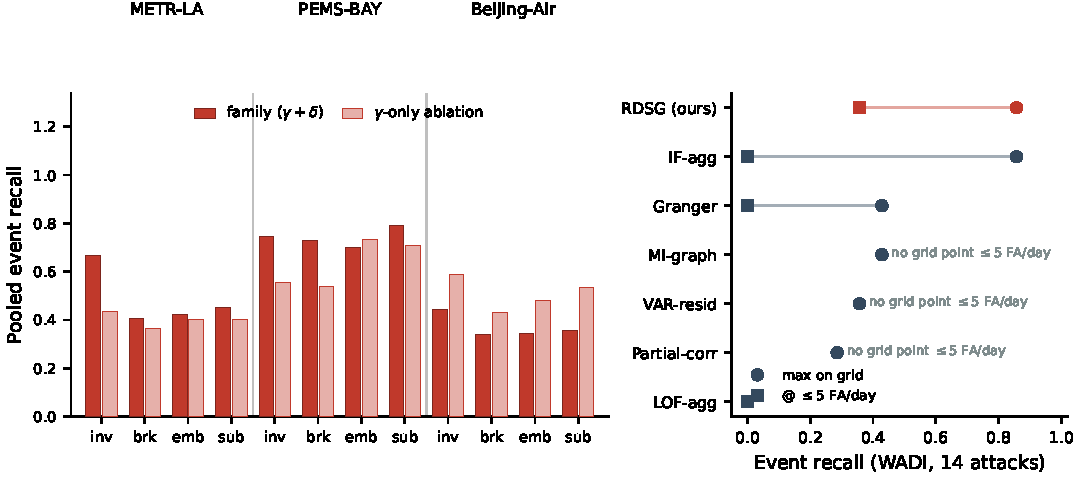
\includegraphics[width=\linewidth]{figs/s12_type_wadi.pdf}
\caption{(a) Pooled event recall by injection type (inv, brk, emb,
sub = subset-joint) on the three networks: family ($\gamma+\delta$,
solid) vs.\ $\gamma$-only ablation (light). (b) WADI: maximum recall on
the sampled operating grid (circles) and recall at $\le 5$ FA/day
(squares); three methods have no sampled operating point at that budget.}
\label{fig:s12}
\end{figure}

\begin{table}[h]\centering\small
\caption{Traceability: pooled per-type recalls behind
Figure~\ref{fig:s12}(a), aggregated from the frozen per-seed files
(\texttt{pooled\_by\_type.json} in the repository).}
\label{tab:s12}
\begin{tabular}{@{}llcccc@{}}
\toprule
Network & Encoding & inv & brk & emb & sub \\
\midrule
METR-LA & family & 0.67 & 0.40 & 0.42 & 0.45 \\
METR-LA & $\gamma$-only & 0.43 & 0.37 & 0.40 & 0.40 \\
PEMS-BAY & family & 0.74 & 0.73 & 0.70 & 0.79 \\
PEMS-BAY & $\gamma$-only & 0.56 & 0.54 & 0.73 & 0.71 \\
Beijing-Air & family & 0.44 & 0.34 & 0.34 & 0.36 \\
Beijing-Air & $\gamma$-only & 0.59 & 0.43 & 0.48 & 0.54 \\
\bottomrule

\end{tabular}
\end{table}

\section*{S.13 Robustness audit of the standardisation constants}

The copula standardisation carries two constants --- the additive
smoothing $\alpha$ and the number of IPF iterations --- that S.8 lists
as untuned design defaults. This audit pre-committed a full grid,
$\alpha\in\{2,4,8,16,32\}\times$ IPF iterations $\in\{1,2,4,8\}$, on the
synthetic gate under the same two-seed single-detector protocol as the
$K\times w$ sweep of the main text's \S5.6 (so absolute recalls are
comparable within, not across, protocols), with the whole pipeline ---
candidate graph, statistics, and self-scan calibration --- running
coherently under each cell's constants. The default ($\alpha{=}8$, two
iterations) was fixed before the audit and is not reselected here; the
main-text numbers are frozen regardless of the outcome.

\begin{table}[h]\centering\small
\caption{Event recall on the pre-committed grid (synthetic gate, two
seeds per cell; the frozen default is $\alpha{=}8$, two iterations).
Realised test-segment FA/day spans $0.36$--$1.04$ across cells,
consistent with the reference-to-test migration of the self-scan rule,
which every cell applies identically.}
\label{tab:s13}
\begin{tabular}{@{}lcccc@{}}
\toprule
$\alpha$ \textbackslash IPF iterations & 1 & 2 & 4 & 8 \\
\midrule
2 & 0.42 & 0.43 & 0.43 & 0.43 \\
4 & 0.47 & 0.53 & 0.53 & 0.50 \\
8 & 0.48 & 0.50 & 0.50 & 0.50 \\
16 & 0.60 & 0.53 & 0.53 & 0.53 \\
32 & 0.50 & 0.53 & 0.53 & 0.53 \\
\bottomrule

\end{tabular}
\end{table}

Recall moves smoothly over $0.425$--$0.600$ across the entire grid with
no cliff anywhere: varying the IPF iterations at the default $\alpha$
shifts recall by at most $0.025$ ($0.475$--$0.500$), and varying
$\alpha$ at two iterations by at most $0.10$ ($0.425$--$0.525$). The
frozen default sits mid-range, and the audit found \emph{better} cells
($\alpha{=}16$ reaches $0.600$) that we do not adopt --- the strongest
available evidence that the reported configuration was not selected for
peak performance. Together with the $K\times w$ sweep of \S5.6 this
extends ``family design, not a lucky hyperparameter'' to every constant
of the standardisation step.

\medskip
\noindent\textbf{Addendum: the real-network audit.} The grid above runs
on the synthetic gate. On METR-LA, under the same protocol with real
hosts (reference-$\gamma$ quantile strata, seeds 1--2, eight cells
spanning $\alpha\in\{2,\dots,32\}$ at two iterations and
$\alpha{=}8$ at $\{1,4,8\}$ iterations), recall spans $0.33$--$0.46$,
with the frozen default ($\alpha{=}8$, two iterations, $0.35$) inside
a flat region: across $\alpha\in\{4,\dots,32\}$ at two iterations
every cell lies within $\pm 0.03$ of the default, and across the IPF
iteration counts the cells span $0.35$--$0.41$; no adjacent pair of
cells differs by more than $0.09$, so there is no cliff. As on the synthetic gate, the audit again finds a \emph{better}
cell that we do not adopt (lightest smoothing, $\alpha{=}2$, reaches
$0.46$ by preserving more signal on genuinely strong real dependencies)
--- the default is not a selected peak
(script \texttt{run\_e5c\_realnet.py}, frozen JSON
\texttt{e5c\_realnet.json} in the repository).

\clearpage
\section*{S.14 Do the deep arms close the gap when trained longer?}

The main text discloses that the Anomaly-Transformer and TranAD rows are
compact reimplementations (official AT architecture; simplified losses; five epochs), which \emph{could} under-train them. This audit
tests that question empirically. Pre-registered design: both arms are
re-run with four times the model width ($d_{\mathrm{model}}{=}256$,
3 layers, 8 heads), thirty epochs with early stopping (patience 5,
last-15\% window-level validation split of the reference segment), the
AT arm still on the official architecture (compact arms: ten seeds,
long arms: five seeds); everything else --- the injection protocol,
seeds, rate-based calibration, event matching ---
is identical to the frozen evaluation. The interpretation rule was fixed
before running: whatever the outcome, it is reported here verbatim.

\begin{table}[h]\centering\small
\caption{Compact arms (frozen, main tables) versus longer-training,
larger-capacity arms (this audit; five seeds each). RDSG column: frozen
family recall (ten seeds), for reference. Longer training does not
close the gap on any network.}
\label{tab:s14}
\begin{tabular}{@{}llccc@{}}
\toprule
Network & Arm & Compact & Long & RDSG \\
\midrule
METR-LA & AT & 0.19 & 0.21 & 0.46 \\
 & TranAD & 0.13 & 0.14 &  \\
PEMS-BAY & AT & 0.21 & 0.21 & 0.57 \\
 & TranAD & 0.22 & 0.21 &  \\
Beijing-Air & AT & 0.08 & 0.06 & 0.23 \\
 & TranAD & 0.14 & 0.16 &  \\
\bottomrule

\end{tabular}
\end{table}

Every compact-to-long change is within $\pm 0.03$ recall (largest:
Beijing-Air TranAD $0.14\to 0.16$), against family leads over the best long
arm of $0.25$ (METR-LA), $0.36$ (PEMS-BAY) and $0.07$ (Beijing-Air,
where the Gaussian-style reading dominates in any case). Early stopping never fired (the validation
loss was still improving slowly at epoch 30), so these are 30-epoch
results rather than converged ones, and the compact-versus-long
differences above are ten-seed versus five-seed means. The ordering
the main text reports is unchanged under this audit:
value-reconstruction and association-discrepancy scorers remain far
below the family on the injection networks at a matched budget. We do not claim official-configuration
status for these arms (the losses remain the disclosed simplified
forms); the claim is narrower and sufficient: this larger-capacity,
thirty-epoch audit does not flip the ordering (script \texttt{run\_abl\_long.py}, frozen JSON
\texttt{abl\_long.json}).

\medskip
\noindent\textbf{Convergence audit.} A second audit extends both long
arms to a 300-epoch cap with early-stopping patience 30, on the same
protocol (five seeds, three networks; script \texttt{run\_abl\_conv.py},
frozen JSON \texttt{abl\_conv.json}). The patience never fires: the
validation loss is still improving at the cap, so even these arms are
not formally converged. The ordering is unchanged and the gap does not
close --- AT $0.13{\pm}0.08$ and TranAD $0.11{\pm}0.02$ on METR-LA
against the family's $0.46$; $0.19{\pm}0.04$ and $0.13{\pm}0.07$ on
PEMS-BAY against $0.57$; $0.05{\pm}0.01$ and $0.19{\pm}0.04$ on
Beijing-Air against $0.23$. A tenfold training budget does not move the
deep arms toward the family under this protocol, so under-training is
not the explanation of the gap.

\medskip
\noindent\textbf{Official-objective audit.} A third audit retrains the
Anomaly-Transformer arm with the \emph{official} training objective and
hyperparameters (minimax association-discrepancy loss with $k{=}3$,
official default capacity $512/512$, ReLU, dropout $0.1$, learning rate
$10^{-4}$, early-stopping patience 3; window kept at the protocol's
$128$), scored by the official association discrepancy under the same
rate-matched calibration (script \texttt{run\_abl\_at\_official.py},
frozen JSON \texttt{abl\_at\_official.json}; seeds 1--5, three
networks). The official objective performs \emph{lower} than the
disclosed simplified arm on every network: $0.047{\pm}0.050$ on METR-LA
(family $0.46$), $0.054{\pm}0.043$ on PEMS-BAY ($0.57$), and
$0.049{\pm}0.006$ on Beijing-Air ($0.23$) --- consistent with its
association discrepancy being a point-anomaly objective, for which
margin-preserving relational injections are out of scope. Across the
simplified, ten-times-longer, and official-objective configurations the
ordering never changes.

\section*{S.20 Scope probe: value-dominant public benchmarks}

The main text excludes SWaT/SMD/PSM/MSL with stated cause. To make the
scope claim empirical rather than rhetorical, this probe runs the family
and two representative monitors on public value-dominant suites under
the same $0.25$/day self-scan protocol (scripts
\texttt{run\_smd\_probe.py}, \texttt{run\_probe\_ics.py}; frozen JSONs
\texttt{smd\_probe.json}, \texttt{probe\_ics.json}). Event counts per
suite are small, so the probe reads as a scope check, not a leaderboard.

\begin{table}[h]\centering\small
\caption{Scope probe on value-dominant suites (event recall; realised
FA/day in parentheses; $0.25$/day protocol throughout).}
\label{tab:s20}
\begin{tabular}{lccccc}
\hline
Suite & Events & RDSG & $\gamma$-only & Partial-corr & LOF-agg \\
\hline
SMD m-1-1 & 5 & 0.00 (0.05) & 0.00 & 1.00 (1.01) & 0.80 (0.25) \\
SMD m-1-2 & 7 & 0.00 (0.00) & 0.00 & 0.14 (0.12) & 0.00 (0.00) \\
SMD m-2-1 & 9 & 0.00 (0.00) & 0.00 & 0.00 (0.24) & 0.00 (0.00) \\
BATADAL & 4 & 0.00 (0.00) & 0.00 & 0.50 (0.01) & 0.25 (0.00) \\
PSM & 25 & 0.00 (0.00) & 0.00 & 0.00 (0.00) & 0.08 (0.02) \\
\hline
\end{tabular}
\end{table}

The reading is exactly the division of labour of the selection guide
(S.16): where labelled attacks carry value-level signatures, value
monitors are the right tool (m-1-1: LOF-agg $0.80$ at budget; BATADAL:
partial correlation $0.50$), and the margin-preserving monitor sits at
its declared floor --- a zero that follows from its design scope
(Lemma~1), not from a defect. Where the attacks are subtle for
everyone (m-1-2, m-2-1, PSM), all methods sit at or near zero. None of
these suites supplies margin-preserving relational attacks, so the
probe validates the paper's scope boundary from the outside: a
deployer facing these failure modes should deploy the value monitors,
not this monitor.

\section*{S.15 Scaling: one-time construction versus online cost}

The main text separates the one-off $O(n^2)$ candidate-graph
construction from the per-boundary scan whose cost is set by the edge
budget, not by $n$. Table~\ref{tab:s15} measures both on the two real
networks (40-channel protocol versions) and on synthetic block-correlated
networks at $n$ up to 2000 (runtime measurement only, not a detection
benchmark; single workstation, single thread for the ranking pass).

\begin{table}[h]\centering\small
\caption{Scaling of the deployment costs. Pair ranking and fit are
one-off; the per-boundary scan (the fitted edge set, 104--116 edges, $w{=}128$;
timed step: table construction plus the statistics, granulation done
before timing) runs at every window boundary and stays at millisecond
scale independently of $n$. RSS is the process reading after fit.}
\label{tab:s15}
\begin{tabular}{@{}rlcccc@{}}
\toprule
$n$ & Network & Rank (s) & Fit (s) & Boundary (ms) & RSS (MB) \\
\midrule
40 & METR-LA (real) & 0.1 & 0.1 & 3.0 & 170 \\
40 & PEMS-BAY (real) & 0.1 & 0.1 & 3.3 & 171 \\
500 & synthetic & 15.2 & 6.8 & 1.4 & 260 \\
1000 & synthetic & 44.9 & 67.6 & 5.4 & 444 \\
2000 & synthetic & 232.6 & 133.3 & 2.1 & 1056 \\
\bottomrule

\end{tabular}
\end{table}

The measurements match the complexity account: the quadratic one-off
construction grows from negligible (real networks) to a few minutes at
$n{=}2000$ --- a deployment cost paid once --- while the online scan
stays in the 1--6\,ms range across a fifty-fold range of $n$, because
the edge budget $E$ is a design constant. Memory grows with $n$
(from $0.17$\,GB at $n{=}40$ to $1.1$\,GB at $n{=}2000$). Together
with the Raspberry Pi measurements of \S5.6 this brackets the deployable
regime from both ends (script \texttt{run\_scaling.py}, frozen JSON
\texttt{scaling.json}).

\clearpage
\section*{S.16 A practitioner's selection guide}

The division of labour observed across the experiments, condensed into
monitoring guidance. Every row is grounded in a specific result of the
main text or this supplement; nothing here extends beyond the measured
evidence.

\medskip
\noindent\begin{tabular}{@{}p{0.30\linewidth}p{0.30\linewidth}p{0.32\linewidth}@{}}
\toprule
If your network looks like & Monitor first with & Because \\
\midrule
Weak associations throughout (the air-quality
profile) & Partial-correlation / Gaussian divergence & Nominally
strongest there ($0.24$ vs.\ $0.23$, Table~5, \S6); no measured
incremental gain for RDSG \\
Strong reference associations, fast sampling (the traffic profile) &
RDSG family ($\gamma{+}\delta$) & Gaussian monitors fall to their floors
under the rate budget (Tables~5--6); family $0.46$/$0.57$ vs.\ best
external $0.19$/$0.49$ \\
Attack-dense ICS logs, low-false-alarm regime (WADI-like) & RDSG at
operating curves & Only method with measured nonzero recall at
$\le 5$ FA/day (5/14 attacks) among methods evaluable at that budget \\
Large point deviations dominate (PEMS-BAY-like) & LOF aggregation first
(Table~5) & Point monitors are the right tool when anomalies move marginals
(\S5.3, \S5.4) \\
Events shorter than half the window & Shrink $w$ and recalibrate
(recommended, not validated here) & Recall rises monotonically with
event length; recall drops steeply below $L = w/2$ (0.34--0.45 at
$L \le w/4$ on the traffic networks, 0.09 on Beijing-Air; Table~9,
\S5.6) \\
Thousands of channels & RDSG viable; budget one-off construction &
Online scan is $n$-independent at ms scale; construction is minutes at
$n{=}2000$ (S.15) \\
\bottomrule
\end{tabular}

\clearpage
\section*{S.17 The $\gamma$--$\delta$ plane: window-level view of the case attacks}

Figure~\ref{fig:s17} replots the case-study edge of S.10 at window
level: every $w{=}128$ rolling window (stride 64) becomes one point
$(\gamma,\delta)$ in the plane. Two reading notes keep the scales
honest: the window support ($128$ points) differs from the
full-reference and attack$\pm64$ anchors quoted in the main text and
S.10, so absolute levels sit below those anchors; and the plane is a
mechanism view, not a detector --- no threshold is drawn. The case
attack traverses the plane along an approximately constant-$\gamma$
vertical band from $\delta=+0.4$ to $\delta=-0.4$: dependency
strength conserved, direction reversed, exactly the geometric form of
the inversion blind spot of Proposition~1(i). Normal windows also
occupy this band; the discriminative signal is therefore the
within-edge temporal change (the S.10 trace), not the static
position in the plane. Most other labelled
attacks leave the point cloud unchanged, consistent with the main-text
finding that $50$ of $53$ gas-pipeline attacks carry a point footprint
that value-level monitors catch more directly (\S5.4 of the main
text): the relational signature is the exception, which is why it
needs its own monitor (script \texttt{fig\_s17\_scatter.py} in the
repository).

\begin{figure}[h]\centering
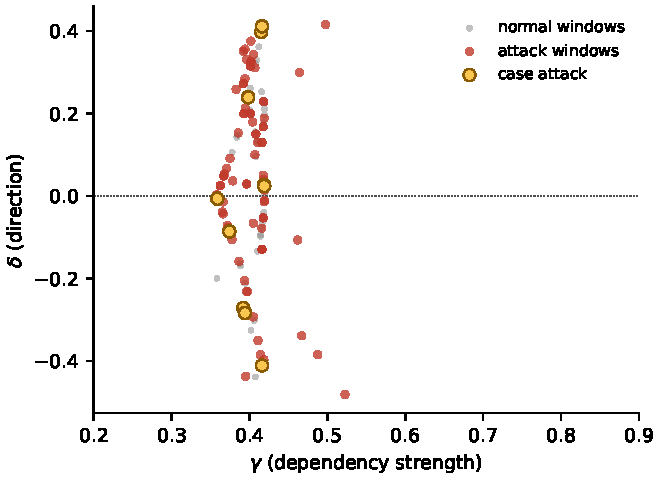
\includegraphics[width=0.72\linewidth]{figs/s17_gd_plane.pdf}
\caption{Window-level $\gamma$--$\delta$ plane of the case-study edge
(setpoint$\to$gain), $w{=}128$ rolling windows over the gas-pipeline
test segment. Grey: normal windows; red: windows overlapping a
labelled attack; yellow with edge: the case attack of \S5.4. The case
traverses an approximately constant-$\gamma$ band across the $\delta$
sign flip (dotted line: $\delta=0$).}
\label{fig:s17}
\end{figure}

\section*{S.18 Data and configuration provenance}

This section records, for every network, the exact channel subset, time
slice and selection rule used by the frozen runs, together with the
complete detection-configuration family; the loaders are
\texttt{rdsg/datasets.py} and \texttt{run\_e2\_oc\_rdsg.py} in the
anonymised repository.

\medskip
\noindent\textbf{Channel subsets and slices.}
\emph{METR-LA:} the released \texttt{metr-la.h5} series, first 34{,}000
rows; channels are the first 40 sensor indices (file order) that are
fully observed (no missing value) over those rows; the first 12{,}000
rows form the reference segment and the next 18{,}000 the test segment
(5-minute sampling).
\emph{PEMS-BAY:} identical rule on \texttt{pems-bay.h5}, first 40{,}000
rows; reference 12{,}000, test 18{,}000.
\emph{Beijing multi-site air quality:} the 12-station PRSA release,
years 2014--2015, the seven sensor variables
PM2.5, PM10, SO$_2$, NO$_2$, O$_3$, TEMP, WSPM (calendar columns
excluded); each station-variable channel is linearly interpolated over
internal gaps, the first 32 fully observed channels are kept, and
channels are reordered variable-major (same variable across stations
adjacent); hourly sampling; the release provides 17{,}520 hourly rows
for 2014--2015, of which the first 12{,}000 form the reference and the
remaining 5{,}520 the test segment.
\emph{MSU gas pipeline:} the nine named process channels (setpoint,
gain, reset rate, deadband, cycle time, rate, pressure measurement, crc
rate, command response), forward/backward filled between polling
responses; the longest clean stretch (27 minutes, rows
238{,}860--240{,}480) is the reference.
\emph{WADI (A2, November 2019):} the top 40 channels by reference
variance, last 12{,}000 reference points at 1-second sampling.

\medskip
\noindent\textbf{Detection-configuration family.} The evaluated family
scans $K\in\{4,2\}$ and $w\in\{128,64,32\}$ points (stride and block
$b=32$); the candidate graph is built once at the primary configuration
($K{=}4$, $w{=}128$): rupture channel top-16 reference-significant
pairs, emergence pool bottom-24 weak pairs plus subset edges over each
weak target's $m{=}6$ closest weak partners, lags
$\tau\in\{0,+1,-1\}$; the boundary grid is the union over the
$(K,w)$ cells at 16-point cadence on the 5-minute networks. The
operating curves are sampled at requested false-alarm budgets of
$\{0.06,0.10,0.15,0.20,0.25,0.40,0.60,1.00\}$ alarm samples per day.
The calibrated $z$-statistics are the left/right window differences of
$\Delta\gamma$ (degree component) and $\Delta\delta$ (direction
component) standardised by the block-permutation nulls of S.8; the
emergence channel scores new dependency on pooled weak edges (formulas
in S.8 and in the main text's calibration section).

\section*{S.19 Random-host audit: injections outside the candidate graph}

The controlled suites of the main text draw injection hosts from the
monitor's own reference-built candidate graph, which invites a
circularity concern: the detector is only asked about edges it monitors.
This audit re-runs the METR-LA suite with hosts drawn \emph{outside} the
candidate graph: INV/BRK hosts from the $390$ non-candidate pairs with
$|$Spearman$|\ge 0.5$, EMB hosts from the $92$ non-candidate weak pairs
($|\rho|<0.3$); ten seeds, ten events per type, identical calibration,
matching rule and length pools (script \texttt{run\_e2f\_ranhost.py},
frozen JSON \texttt{e2f\_ranhost\_metr\_la.json}). Hosts are verified to
lie outside the candidate edge set in every seed.

\begin{table}[h]\centering\small
\caption{Random-host audit (METR-LA, ten seeds): event recall when
injection hosts are drawn outside the candidate graph, against the
candidate-host suite of Table~5 (same protocol, same seeds).}
\label{tab:s19}
\begin{tabular}{lcc}
\hline
Method & Hosts outside graph & Hosts in graph (Table~5) \\
\hline
RDSG (ours) & $0.398\pm0.058$ & $0.456\pm0.05$ \\
Partially-corr & $0.103\pm0.049$ & $0.11\pm0.04$ \\
MI-graph & $0.105\pm0.043$ & $0.09\pm0.03$ \\
Corr-matrix & $0.060\pm0.049$ & $0.07\pm0.03$ \\
IF-agg & $0.050\pm0.086$ & $0.07\pm0.07$ \\
LOF-agg & $0.046\pm0.036$ & $0.04\pm0.03$ \\
\hline
\end{tabular}
\end{table}

Two facts answer the concern. First, the family retains most of its
power on pairs it does not monitor ($0.398$ against $0.456$ on
candidate hosts): on a densely coupled network a structural rupture on
an unmonitored pair propagates to monitored edges, so the fixed graph
acts as a sensor placement, not a blindfold. Second, the baselines that
scan \emph{all} pairs do not improve when the suite leaves the candidate
graph: partial correlation moves $0.11	o0.103$, the correlation
matrix $0.07	o0.060$, and MI-graph $0.09	o0.105$ --- none of the
three leaves its floor region, and the small MI-graph rise merely swaps
its Table~5 order with partial correlation within noise. The family's
advantage over the strongest external baseline of the suite remains
significant (one-sided Wilcoxon, $p=0.001$). The audit covers one
network and margin-preserving injections only; it bounds the
circularity concern for this protocol rather than for all conceivable
host distributions.

\end{document}
